\documentclass[aspectratio=169, 10pt]{beamer}
%\documentclass[handout, 10pt]{beamer}
\usetheme{Berlin}
\usepackage[utf8]{inputenc}
\usepackage[ngerman]{babel}
\usepackage[T1]{fontenc}
\usepackage{amsmath}
\usepackage{amsfonts}
\usepackage{amssymb}
\usepackage{graphicx}
\usepackage{tabularx}
\usepackage{csquotes}
\usepackage{siunitx}
\usepackage{physics}
\usepackage{xfrac}
\usepackage[siunitx]{circuitikz}
\usepackage{textcomp}
\usepackage{mathtools}
\usepackage{siunitx}
%\usepackage{textgreek}
\usepackage{caption}
\usepackage{subfig}
\usepackage{bbold}
\usepackage{makecell}
\usepackage{ulem}
\usepackage{minted}
\usepackage{listings}



\usepackage[style=verbose,backend=bibtex]{biblatex}
\addbibresource{literature.bib}

\hypersetup{colorlinks=true, urlcolor=cyan, linkcolor=white}

%\definecolor{darkred}{hsb}{0.606,0.45,0.50}
\definecolor{darkred}{RGB}{70,91,128}


\setbeamertemplate{navigation symbols}{} 
\setbeamercolor{palette primary}{fg=white,bg=darkred}

%\setbeamercolor{bibliography entry author}{fg=darkred}
%\setbeamercolor{bibliography entry title}{fg=black} 
%\setbeamercolor{bibliography entry location}{fg=gray!70!black} 
%\setbeamercolor{bibliography entry note}{fg=gray!70!black}  

%\setbeamercolor{bibliography entry author}{fg=darkred!70!white}
%\setbeamercolor{bibliography entry title}{fg=white} 
%\setbeamercolor{bibliography entry location}{fg=gray!70!white} 
%\setbeamercolor{bibliography entry note}{fg=gray!70!white}  

\setbeamercolor{itemize item}{fg=darkred,bg=darkred}
\setbeamercolor{description item}{fg=darkred,bg=darkred}
\setbeamercolor{itemize subitem}{fg=darkred,bg=darkred}
\setbeamercolor{itemize subsubitem}{fg=darkred,bg=darkred}
\setbeamercolor{enumerate items}{fg=darkred,bg=darkred}
\setbeamercolor{enumerate subitems}{fg=darkred,bg=darkred}
\setbeamercolor{enumerate subsubitems}{fg=darkred,bg=darkred}
\setbeamercolor{item projected}{bg=darkred}
\setbeamercolor{section in head/foot}{fg=white,bg=darkred}
\setbeamertemplate{section in head/foot shaded}{\color{white!65!black}\usebeamertemplate{section in head/foot}}
\setbeamercolor{author in head/foot}{fg=white,bg=darkred}
\setbeamercolor{section in toc}{fg=black}
\setbeamercolor{caption name}{fg=darkred}
\setbeamertemplate{caption}[numbered]

\let\oldsection\section
\renewcommand{\section}[1]{
	\oldsection{#1}
	\sbgframe{
		\begin{minipage}{.8\textwidth}
			\begin{center}
				\usebeamerfont{part title}\insertsection
			\end{center}
		\end{minipage}
	}{5mm}
	\addtocounter{framenumber}{-1}
}

\sisetup{%
  %locale = DE,
  per-mode = symbol,
  range-phrase = \text{--},
  range-units = single,
  separate-uncertainty = true
}


\let\oldtitle\title
\def\title#1{%
	\oldtitle{#1}
	\def\thetitle{#1}
}
\let\oldsubtitle\subtitle
\def\subtitle#1{%
	\oldsubtitle{#1}
	\def\thesubtitle{#1}
}
\let\oldauthor\author
\def\author#1{%
	\oldauthor{#1}
	\def\theauthor{#1}
}
\let\oldinstitute\institute
\def\institute#1{%
	\oldinstitute{#1}
	\def\theinstitute{#1}
}
\usepackage{datetime}
\newcommand{\datef}[3]{%
  \newdate{datex}{#1}{#2}{#3}
  \date{\protect\displaydate{datex}}
  \def\thedate{\protect\displaydate{datex}}
}


\newcommand{\oldarraystretch}{\relax}
\newenvironment{stretcharrays}[1]{%
    \renewcommand{\oldarraystretch}{\arraystretch}
    \renewcommand{\arraystretch}{#1}
}{%
    \renewcommand{\arraystretch}{\oldarraystretch}
    \renewcommand{\oldarraystretch}{\relax}
}

\makeatletter
\setbeamertemplate{headline}
{%
  \begin{beamercolorbox}[colsep=1.5pt]{upper separation line head}
  \end{beamercolorbox}
  \begin{beamercolorbox}{section in head/foot}
    \vskip2pt\insertsectionnavigationhorizontal{\paperwidth}{}{}\vskip2pt
  \end{beamercolorbox}%
  \vspace*{-1pt}
}
\setbeamertemplate{footline}
{%
	\begin{beamercolorbox}[wd=1.0\textwidth,ht=2.6ex,dp=1ex,leftskip=.5em,rightskip=.5em]{author in head/foot}%
	\usebeamerfont{author in head/foot}%
	\insertshortauthor\hfill%
	\insertframenumber{} / \inserttotalframenumber%
	\end{beamercolorbox}%
	\vspace*{-3.6ex}%
	\begin{beamercolorbox}[wd=1.0\textwidth,ht=2.6ex,dp=1ex,left,leftskip=.5em,rightskip=.5em]{}%
	\color{white}%
	\usebeamerfont{title in head/foot}%
	\phantom{A}%
	\hfill%
	\insertshorttitle\hfill%
	\phantom{A}%
	\end{beamercolorbox}%
}
\makeatother
\setbeamerfont{footline}{series=\bfseries}

\makeatletter
\newlength\beamerleftmargin
\setlength\beamerleftmargin{\Gm@lmargin}
\makeatother

\setlength{\belowcaptionskip}{-10pt}




\newcommand{\bgframe}[2]{%
	\begin{frame}[plain]%
	\vspace*{0.5cm}%
	\makebox[\textwidth][c]{%
		\begin{tikzpicture}%
		    \node[minimum width=1.1\paperwidth,%
		          minimum height=1.1\paperheight,%
		          anchor=north west] (a) {%
			    \includegraphics[height=0.4\paperheight]{Bilder/Git-logo.pdf}%geaendert
		    };%
			\node[fill=black,%
			      fill opacity=0.7,%
			      text opacity=1,%
			      draw opacity=1,%
			      inner sep=5mm,%
			      at=(a.center),%
			      yshift={#2}] {\color{white}{#1}};%
		\end{tikzpicture}%
	}%
	\end{frame}%
}

\newcommand{\sbgframe}[2]{%
	\begin{frame}<handout:0>[plain]%
	\vspace*{-2mm}%
	\makebox[\textwidth][c]{%
		\begin{tikzpicture}%
		    \node[minimum width=1.1\paperwidth,%
		          minimum height=1.1\paperheight,%
		          anchor=north west] (a) {%
			    \includegraphics[height=0.4\paperheight]{Bilder/Git-logo.pdf}%geaendert
		    };%
			\node[fill=black,%
			      fill opacity=0.7,%
			      text opacity=1,%
			      draw opacity=1,%
			      inner sep=5mm,%
			      at=(a.center),%
			      yshift={#2}] {\color{white}{#1}};%
		\end{tikzpicture}%
	}%
	\end{frame}%
}

\newcommand{\bluearrow}{{\color{darkred}\(\boldsymbol{\Rightarrow}\)}}

\newcommand{\arrowitem}{\item[\bluearrow\hspace*{-1pt}]}

\newcommand\ddfrac[2]{\frac{\displaystyle #1}{\displaystyle #2}}


%geaendert
\title{13 Git Visualisierung}
\subtitle{Python Grundkurs}
\author{Sven Bollweg, Bogdan Wiederspan}
\institute{Universität Hamburg}
\datef{30}{01}{2024}





\begin{document}

\bgframe{
	\shortstack{
		\LARGE
		\thetitle
		\\
		\thesubtitle
		\\[5mm]
		\theauthor
		\\[5mm]
	}
}{4cm}



\begin{frame}{Überblick über lokale und remote Repositories}

	\begin{figure}
		\begin{center}
			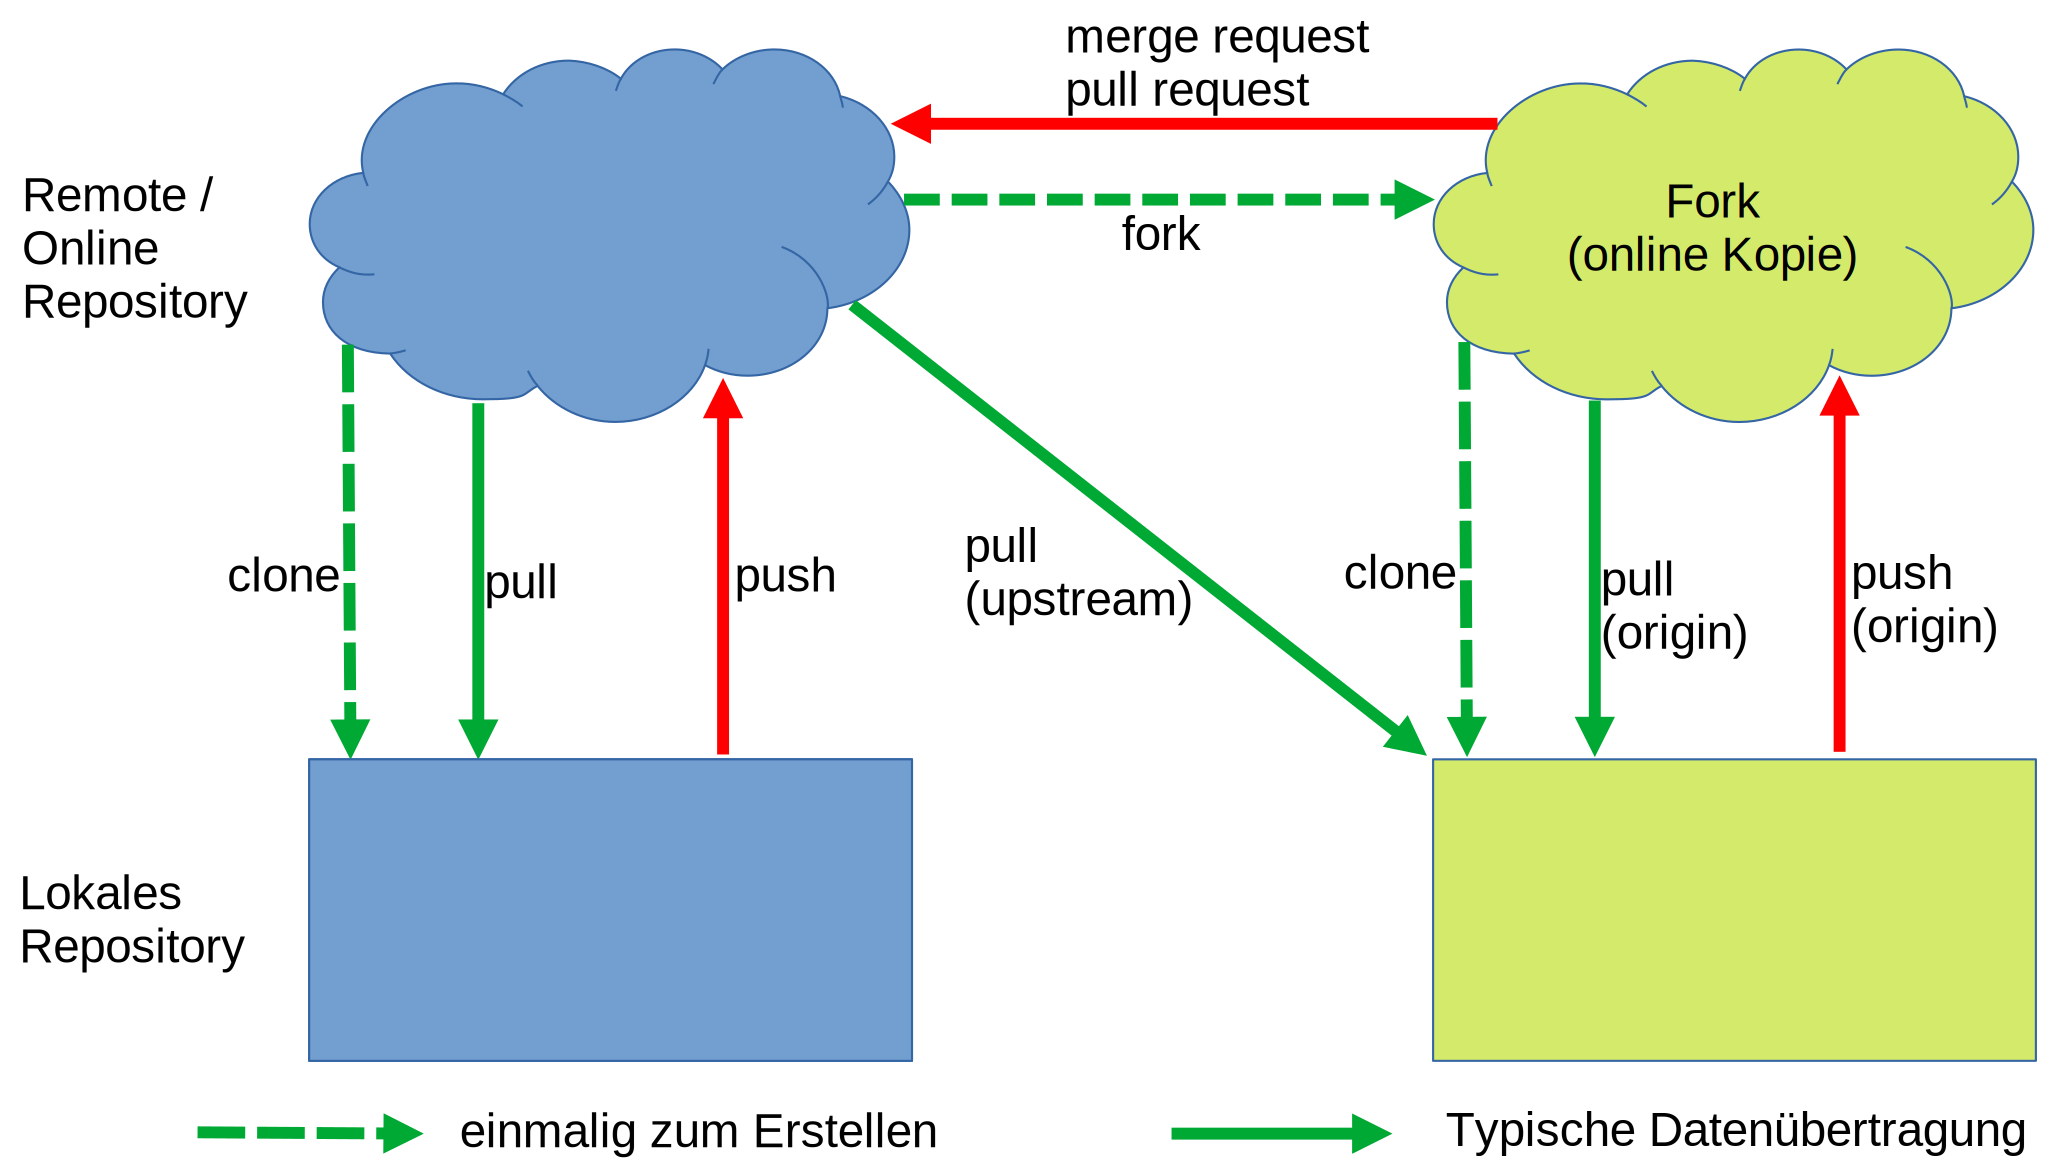
\includegraphics[width=0.8\textwidth]{Bilder/Git_lokal_remote.pdf}
		\end{center}
	\end{figure}

\end{frame}


\begin{frame}{lokales Rpository}

	Ab jetzt betrachten wir ein lokales Repository

\end{frame}


\begin{frame}{Aufbau}

	\only<1>{
	\begin{figure}
		\begin{center}
			\includegraphics[width=\textwidth]{Bilder/Git_Visualisierung_1.pdf}
		\end{center}
	\end{figure}}
	
	\only<2>{
	\begin{figure}
		\begin{center}
			\includegraphics[width=\textwidth]{Bilder/Git_Visualisierung_2.pdf}
		\end{center}
	\end{figure}}
	
	\only<3>{
	\begin{figure}
		\begin{center}
			\includegraphics[width=\textwidth]{Bilder/Git_Visualisierung_3.pdf}
		\end{center}
	\end{figure}}
	
	\only<4>{
	\begin{figure}
		\begin{center}
			\includegraphics[width=\textwidth]{Bilder/Git_Visualisierung_4.pdf}
		\end{center}
	\end{figure}}
	
	%\onslide<3->{
	\begin{overlayarea}{\textwidth}{2cm}
		\only<3>{Pfeilrichtung in Zeitrichtung}
		\only<4->{Technische Pfeilrichtung: Für jeden Commit ist der einzige Vorgänger bekannt (Ausnahme Merge Commit \(\rightarrow\) siehe später)}
	\end{overlayarea}

\end{frame}


\begin{frame}{Commit erstellen}

	\only<1>{
	\begin{figure}
		\begin{center}
			\includegraphics[width=\textwidth]{Bilder/Git_Visualisierung_4.pdf}
		\end{center}
	\end{figure}}
	
	\only<2->{
	\begin{figure}
		\begin{center}
			\includegraphics[width=\textwidth]{Bilder/Git_Visualisierung_5.pdf}
		\end{center}
	\end{figure}}
	
	\vspace{-1cm}
	
	\begin{overlayarea}{\textwidth}{3cm}
		\begin{itemize}
			\item Befehl: \mintinline{bash}{git commit}
			\item<2-> Erstellt neuen Commit und setzt den zuletzt aktuellen Commit als Vorgänger
			\item<2-> Verschiebt HEAD und aktuellen Branch auf den neuen Commit
		\end{itemize}
	\end{overlayarea}

\end{frame}


\begin{frame}{Neuen Branch erstellen}

	\only<1>{
	\begin{figure}
		\begin{center}
			\includegraphics[width=\textwidth]{Bilder/Git_Visualisierung_5.pdf}
		\end{center}
	\end{figure}}
	
	\only<2,3>{
	\begin{figure}
		\begin{center}
			\includegraphics[width=\textwidth]{Bilder/Git_Visualisierung_6.pdf}
		\end{center}
	\end{figure}}
	
	\only<4>{
	\begin{figure}
		\begin{center}
			\includegraphics[width=\textwidth]{Bilder/Git_Visualisierung_7.pdf}
		\end{center}
	\end{figure}}
	
	\begin{overlayarea}{\textwidth}{2cm}
		\only<1,2>{
		\begin{itemize}
			\item<1,2> \mintinline{bash}{git branch feature1}
			\item<2> Erzeugt einen neuen Branch mit dem Namen \mintinline{bash}{feature1} am aktuellen Commit
		\end{itemize}}
		\only<3>{
		\begin{itemize}
			\item Um auf den neuen Branch zu arbeiten, muss dorthin gewechselt werden
			\item \mintinline{bash}{git checkout feature1}
		\end{itemize}}
		\only<4>{Ein neuer Commit auf \mintinline{bash}{feature1}}
	\end{overlayarea}

\end{frame}


\begin{frame}{Branch mergen (fast forward)}

	\only<1>{
	\begin{figure}
		\begin{center}
			\includegraphics[width=\textwidth]{Bilder/Git_Visualisierung_7.pdf}
		\end{center}
	\end{figure}}
	
	\only<2,3>{
	\begin{figure}
		\begin{center}
			\includegraphics[width=\textwidth]{Bilder/Git_Visualisierung_8.pdf}
		\end{center}
	\end{figure}}
	
	\only<4>{
	\begin{figure}
		\begin{center}
			\includegraphics[width=\textwidth]{Bilder/Git_Visualisierung_9.pdf}
		\end{center}
	\end{figure}}
	
	\vspace{-0.5cm}
	
	\begin{overlayarea}{\textwidth}{3cm}
		\only<1,2>{
		\begin{itemize}
			\item Soll in \mintinline{bash}{master} gemerged werden \(\rightarrow\) wir müssen auf \mintinline{bash}{master} sein
			\item \mintinline{bash}{git checkout master}
		\end{itemize}}
		
		\only<3,4>{
		\begin{itemize}
			\item mergen von \mintinline{bash}{feature1} in \mintinline{bash}{master}
			\item \mintinline{bash}{git merge feature1}
			\item<4> fast forward merge: Verschieben des \mintinline{bash}{master} Labels auf \mintinline{bash}{feature1}
		\end{itemize}}
	\end{overlayarea}

\end{frame}


\begin{frame}{Arbeiten mit mehreren Branches}

	\only<1>{
	\begin{figure}
		\begin{center}
			\includegraphics[width=\textwidth]{Bilder/Git_Visualisierung_9.pdf}
		\end{center}
	\end{figure}}
	
	\only<2>{
	\begin{figure}
		\begin{center}
			\includegraphics[width=\textwidth]{Bilder/Git_Visualisierung_10.pdf}
		\end{center}
	\end{figure}}
	
	\only<3>{
	\begin{figure}
		\begin{center}
			\includegraphics[width=\textwidth]{Bilder/Git_Visualisierung_11.pdf}
		\end{center}
	\end{figure}}
	
	\only<4,5>{
	\begin{figure}
		\begin{center}
			\includegraphics[width=\textwidth]{Bilder/Git_Visualisierung_12.pdf}
		\end{center}
	\end{figure}}
	
	\only<6>{
	\begin{figure}
		\begin{center}
			\includegraphics[width=\textwidth]{Bilder/Git_Visualisierung_13.pdf}
		\end{center}
	\end{figure}}
	
	\begin{overlayarea}{\textwidth}{3cm}
		\only<2>{
		\begin{itemize}
			\item ein neuer Commit auf \mintinline{bash}{feature1} wurde erstellt
			\item zurück gewechselt auf \mintinline{bash}{master}
		\end{itemize}}
		
		\only<3>{
		\begin{itemize}
			\item neuer Branch \mintinline{bash}{feature2} wurde erstellt
			\item auf \mintinline{bash}{feature2} gewechsel
		\end{itemize}}
		
		\only<4>{
		\begin{itemize}
			\item neuer Commit auf \mintinline{bash}{feature2}
		\end{itemize}}
		
		\only<5>{
		\begin{itemize}
			\item sowohl \mintinline{bash}{feature1} als auch \mintinline{bash}{feature2} basieren beide auf Commit \mintinline{bash}{5} bzw. \mintinline{bash}{master}
			\item beide Branches können unabhängig voneinander und \glqq zeitgleich\grqq\ entwickelt werden
		\end{itemize}}
		
		\only<6>{
		\begin{itemize}
			\item \mintinline{bash}{feature1} wurde in \mintinline{bash}{master} gemerged (fast forward merge)
		\end{itemize}}
	\end{overlayarea}

\end{frame}


\begin{frame}{Branch mergen (merge Commit)}

	\only<1>{
	\begin{figure}
		\begin{center}
			\includegraphics[width=\textwidth]{Bilder/Git_Visualisierung_13.pdf}
		\end{center}
	\end{figure}}
	
	\only<2,3,4>{
	\begin{figure}
		\begin{center}
			\includegraphics[width=\textwidth]{Bilder/Git_Visualisierung_14.pdf}
		\end{center}
	\end{figure}}
	
	\only<5>{
	\begin{figure}
		\begin{center}
			\includegraphics[width=\textwidth]{Bilder/Git_Visualisierung_15.pdf}
		\end{center}
	\end{figure}}
	
	\vspace{-0.2cm}
	
	\begin{overlayarea}{\textwidth}{3cm}
		\only<1>{
		\begin{itemize}
			\item \mintinline{bash}{feature2} soll in \mintinline{bash}{master} gemerged werden
			\item wechseln auf den \mintinline{bash}{master} branch: \mintinline{bash}{git checkout master}
		\end{itemize}}
		
		\only<3>{
		\begin{itemize}
			\item Problem: \mintinline{bash}{feature2} basiert nicht auf dem aktuellsten Commit von \mintinline{bash}{master} \(\rightarrow\) fast forward (Verschieben des \mintinline{bash}{master} Labels auf \mintinline{bash}{feature2}) nicht möglich %(Verlust der \mintinline{bash}{feature1} Entwicklungen
			\item brauchen merge Commit zum zusammenführen
		\end{itemize}}
		
		\only<4,5>{
		\begin{itemize}
			\item Befehl: \mintinline{bash}{git merge feature2}
			\item<5> Merge Commit: hat zwei Vorgänger: ehemaliger Stand des aktuellen Branches (\mintinline{bash}{master}) und des gemergedten Branches (\mintinline{bash}{feature2})
		\end{itemize}}
	\end{overlayarea}

\end{frame}


\begin{frame}{In die Vergangenheit reisen}

	\only<1-3,8>{
	\begin{figure}
		\begin{center}
			\includegraphics[width=\textwidth]{Bilder/Git_Visualisierung_15.pdf}
		\end{center}
	\end{figure}}
	
	\only<4-7>{
	\begin{figure}
		\begin{center}
			\includegraphics[width=\textwidth]{Bilder/Git_Visualisierung_16.pdf}
		\end{center}
	\end{figure}}
	
	\vspace{-0.2cm}
	
	\begin{overlayarea}{\textwidth}{3cm}
		\only<1>{
		\begin{itemize}
			\item \mintinline{bash}{git checkout <branchname>}
			\item ermöglicht Reisen zu \glqq veralteten\grqq\ Branches
		\end{itemize}}
		
		\only<2>{
		\begin{itemize}
			\item \mintinline{bash}{git checkout HEAD~<Anzahl Commits>} Setzt HEAD um gegebene Zahl zurück (Achtung merge Commits)
			\item \mintinline{bash}{git checkout <Commit Hash>} Ziel Commit anhand des Hashes festlegen
		\end{itemize}}
		
		\only<3,4>{
		\begin{itemize}
			\item \mintinline{bash}{git checkout 4}
			\item<4> detached HEAD: HEAD ist keinem Branch zugewiesen, es kann nur eingeschränkt gearbeitet werden
		\end{itemize}}
		
		\only<5,6>{
		\begin{itemize}
			\item Wie kommt man zurück? Infos über Nachfolger nicht vorhanden
			\item<6> Branches
		\end{itemize}}
		
		\only<7,8>{
		\begin{itemize}
			\item \mintinline{bash}{git checkout master}
		\end{itemize}}
	\end{overlayarea}

\end{frame}




\newcounter{savedframenumber}
\setcounter{savedframenumber}{\theframenumber}

%\section*{Backup}





\setcounter{framenumber}{\thesavedframenumber}

\end{document}